\documentclass[11pt]{article}

\usepackage[margin=1in]{geometry}
\usepackage{amsmath,amssymb,amsthm}
\usepackage{graphicx}
\usepackage[hidelinks]{hyperref}

\newtheorem{theorem}{Theorem}
\newtheorem{lemma}{Lemma}

\newcommand{\Buo}{\mathsf{Buo}}
\newcommand{\uo}{\mathsf{uo}}
\newcommand{\ellp}{\ell_p}
\newcommand{\ellone}{\ell_1}
\newcommand{\sgn}{\operatorname{sgn}}

\title{Bourgain-root counterexamples to sequential \texorpdfstring{\(\Buo\)}{Buo} completeness of \texorpdfstring{\(\ell_p\)}{ell p}}
\author{Run \texttt{fa\_banach\_001}, lane 7}
\date{2026-06-16}

\begin{document}
\maketitle

\section*{Status}

This packet records a candidate counterexample to the \(\ell_p\) bullet in
Question 5.2 of Kania and Swaczyna's paper
\emph{Bourgain--uo sequential completeness in vector lattices}
\cite{KaniaSwaczyna}.  The source asks whether \(\Buo\)-Cauchy sequences
converge in \(\ell_p\) for \(1<p<\infty\).  We show that the answer is
negative for every \(1<p<\infty\).

The construction uses Bourgain's 1981 counterexample in \(\ell_1\)
\cite{Bourgain1981} and a coordinatewise \(p\)-root transform.  The new point
is that this transform preserves the relevant subsequence-difference Cauchy
condition while turning \(\ell_1\)-domination into \(\ell_p\)-domination.

\section*{Source Question}

The open question appears on page 12 of the source PDF.

\begin{center}

\includegraphics[width=\textwidth]{figures/open_problem_crop.png}
\end{center}

The relevant bullet asks whether \(\Buo\)-Cauchy sequences converge in
\(\ell_p\) for \(1<p<\infty\).

\section*{Bourgain's Input}

Bourgain considers on \(\ell_1\) the convergence given by coordinatewise
convergence plus domination by a single element of \(\ell_1\).  For sequences
in \(\ell_1\), this is exactly order convergence.  He calls a sequence Cauchy
when the consecutive differences along every increasing subsequence converge
in this sense, and proves that there is such a Cauchy sequence which is not
convergent in this sense \cite[p.~175]{Bourgain1981}.

\begin{center}
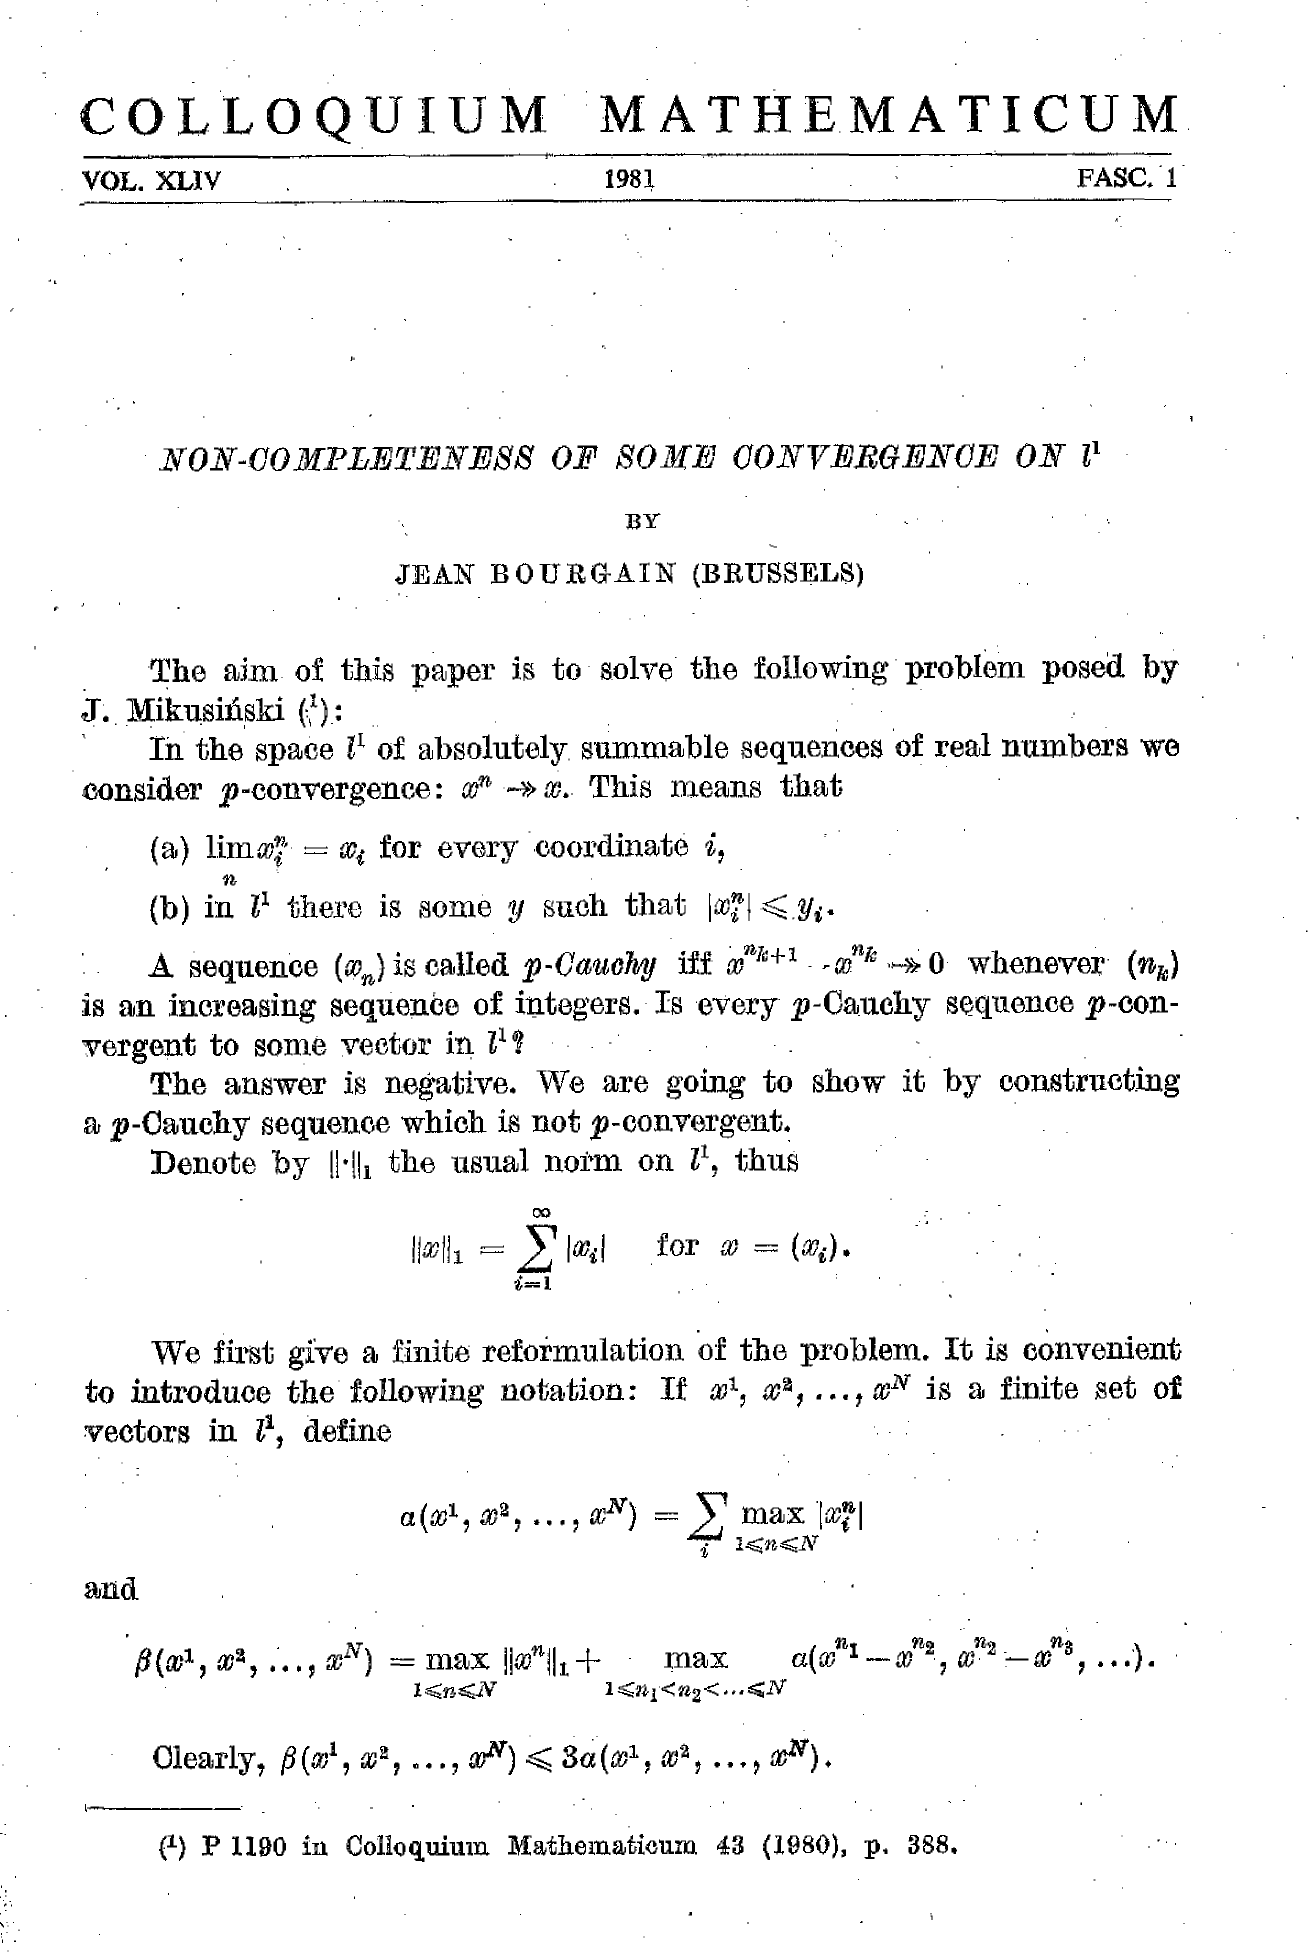
\includegraphics[width=.86\textwidth]{figures/bourgain_definition_page.png}
\end{center}

In the terminology of Kania and Swaczyna, Bourgain's result gives a
\(\Buo\)-Cauchy sequence \((z_n)\) in \(\ell_1\) which does not converge in
order in \(\ell_1\).

\section*{Proof Intuition}

The obstruction in Bourgain's example is not tied to the linear structure of
\(\ell_1\); it is tied to domination.  The coordinatewise map
\[
        \Phi_p(t)=\sgn(t)|t|^{1/p}
\]
converts \(\ell_1\)-summability of a positive sequence into
\(\ell_p\)-summability of its \(p\)-root.  It is also Hölder:
small dominated differences in \(\ell_1\) become small dominated differences
in \(\ell_p\).  Thus Bourgain's Cauchy property survives the transform.
Conversely, if the transformed sequence were order convergent in \(\ell_p\),
raising coordinates back to the \(p\)th power would make Bourgain's original
sequence order convergent in \(\ell_1\), which is impossible.

\section*{A Root-Map Lemma}

\begin{lemma}\label{lem:root-preserves-cauchy}
Let \(1<p<\infty\), and define
\[
        \Phi_p(t)=\sgn(t)|t|^{1/p}\qquad(t\in\mathbb R).
\]
If \(a_m-b_m\to0\) in order in \(\ell_1\), then
\[
        \Phi_p(a_m)-\Phi_p(b_m)\to0
\]
in order in \(\ell_p\), where \(\Phi_p\) is applied coordinatewise.
\end{lemma}

\begin{proof}
For real \(s,t\) one has
\[
        |\Phi_p(s)-\Phi_p(t)|^p \le 2^{p-1}|s-t|.
\]
Indeed, if \(s\) and \(t\) have the same sign this follows from the
\(1/p\)-Hölder continuity of \(u\mapsto u^{1/p}\) on \([0,\infty)\).  If they
have opposite signs, then concavity gives
\[
|\Phi_p(s)-\Phi_p(t)|
        = |s|^{1/p}+|t|^{1/p}
        \le 2^{1-1/p}(|s|+|t|)^{1/p}
        = 2^{1-1/p}|s-t|^{1/p}.
\]

Since \(a_m-b_m\to0\) in order in \(\ell_1\), there are positive
\(\ell_1\)-vectors \(w_\alpha\downarrow0\) such that, for every \(\alpha\),
\[
        |a_m-b_m|\le w_\alpha
\]
eventually in \(m\).  The displayed scalar estimate gives
\[
        |\Phi_p(a_m)-\Phi_p(b_m)|
        \le 2^{1-1/p} w_\alpha^{1/p}
\]
eventually, where the root is taken coordinatewise.  Since
\((w_\alpha^{1/p})^p=w_\alpha\in\ell_1\), we have
\(w_\alpha^{1/p}\in\ell_p\), and \(w_\alpha^{1/p}\downarrow0\) coordinatewise.
Thus the transformed differences converge to \(0\) in order in \(\ell_p\).
\end{proof}

\section*{Counterexample}

\begin{theorem}
For every \(1<p<\infty\), \(\ell_p\) is not sequentially
\(\Buo\)-complete.  Equivalently, there is a \(\Buo\)-Cauchy sequence in
\(\ell_p\) which does not converge in order, and hence does not
\(\Buo\)-converge.
\end{theorem}

\begin{proof}
Let \((z_n)\subset\ell_1\) be Bourgain's sequence: it is Cauchy for the
subsequence-difference convergence described above, but it is not convergent
for coordinatewise-plus-\(\ell_1\)-dominated convergence.  Since that
convergence is order convergence in \(\ell_1\), \((z_n)\) is \(\Buo\)-Cauchy
in \(\ell_1\) but not order convergent.

Fix \(1<p<\infty\), and define
\[
        x_n(j)=\Phi_p(z_n(j))
        =\sgn(z_n(j))|z_n(j)|^{1/p}\qquad(j\in\mathbb N).
\]
Then \(x_n\in\ell_p\), because
\[
        \|x_n\|_p^p=\sum_j |x_n(j)|^p
        =\sum_j |z_n(j)|=\|z_n\|_1<\infty.
\]

We first show that \((x_n)\) is \(\Buo\)-Cauchy in \(\ell_p\).  Let
\((n_k)\) be any strictly increasing sequence.  Since \((z_n)\) is
\(\Buo\)-Cauchy in \(\ell_1\),
\[
        z_{n_{k+1}}-z_{n_k}\to0
\]
in order in \(\ell_1\).  Applying Lemma~\ref{lem:root-preserves-cauchy} with
\(a_k=z_{n_{k+1}}\) and \(b_k=z_{n_k}\), we obtain
\[
        x_{n_{k+1}}-x_{n_k}
        =\Phi_p(z_{n_{k+1}})-\Phi_p(z_{n_k})\to0
\]
in order in \(\ell_p\).  Since \((n_k)\) was arbitrary, \((x_n)\) is
\(\Buo\)-Cauchy in \(\ell_p\).

It remains to show that \((x_n)\) is not order convergent in \(\ell_p\).
Suppose otherwise.  Then \(x_n\to x\) in order for some \(x\in\ell_p\).
Order convergence in \(\ell_p\) implies coordinatewise convergence and
eventual domination: after discarding finitely many terms, there is
\(y\in(\ell_p)_+\) with \(|x_n|\le y\).  Define
\[
        \Psi_p(t)=\sgn(t)|t|^p.
\]
Coordinatewise, \(z_n=\Psi_p(x_n)\), and \(z_n(j)\to\Psi_p(x(j))\).  Moreover
\[
        |z_n(j)|=|x_n(j)|^p\le y(j)^p,
\]
and \(y^p\in\ell_1\), for all sufficiently large \(n\).  Adding the finitely
many initial vectors \(|z_1|,\ldots,|z_{N-1}|\) to this dominator gives one
element of \(\ell_1\) dominating the whole sequence.  Therefore \((z_n)\)
converges in the coordinatewise-plus-\(\ell_1\)-dominated sense, equivalently
in order in \(\ell_1\).  This contradicts Bourgain's choice of \((z_n)\).

Thus \((x_n)\) is a \(\Buo\)-Cauchy sequence in \(\ell_p\) which does not
converge in order.
\end{proof}

\section*{Compatibility with the Norm-Convergence Packet}

A separate packet in this run proves that every \(\Buo\)-Cauchy sequence in
\(\ell_p\), \(1\le p<\infty\), is norm Cauchy and hence norm convergent.  The
present counterexample is compatible with that result: it rules out the
stronger conclusion of order convergence, not norm convergence.

\section*{Novelty and Literature Check}

The supporting literature used here is Bourgain's 1981 paper
\cite{Bourgain1981}, located through Crossref DOI
\href{https://doi.org/10.4064/cm-44-1-175-178}{10.4064/cm-44-1-175-178} and
downloaded from the IMPAN publication page.  Page 175 contains the relevant
definition of the Cauchy condition and the negative answer in \(\ell_1\).

Searches for exact phrases around ``Bourgain--uo'', ``\(\Buo\)-Cauchy'',
``\(\ell_p\)'', and the source question surfaced the source paper and adjacent
bounded-\(\uo\) completeness material, but no later explicit resolution of the
\(\ell_p\) bullet.  The counterexample is best viewed as a short transfer
argument from Bourgain's \(\ell_1\) construction; novelty confidence is
therefore moderate, and human review should check whether this root-map
transfer is already known or implicit in unpublished notes.

\section*{Human Review Recommendation}

Check two points:
\begin{enumerate}
\item Bourgain's Cauchy condition on page 175 is exactly the
      subsequence-difference order convergence condition used here.
\item The scalar Hölder estimate in Lemma~\ref{lem:root-preserves-cauchy}
      correctly transports order-null difference sequences from \(\ell_1\) to
      \(\ell_p\).
\end{enumerate}
If both checks pass, the \(\ell_p\) bullet of Question 5.2 is answered
negatively for every \(1<p<\infty\).

\begin{thebibliography}{9}

\bibitem{Bourgain1981}
J.~Bourgain,
\newblock \emph{Non-completeness of some convergence on \(\ell^1\)},
\newblock Colloquium Mathematicum \textbf{44} (1981), no.~1, 175--178,
\newblock DOI: \href{https://doi.org/10.4064/cm-44-1-175-178}{10.4064/cm-44-1-175-178}.

\bibitem{KaniaSwaczyna}
T.~Kania and J.~Swaczyna,
\newblock \emph{Bourgain--uo sequential completeness in vector lattices},
\newblock arXiv:2512.14949, 2025.

\end{thebibliography}

\end{document}
